\section{Scopo e strumentazione}

Scopo di quest'esperienza è il realizzare un amplificatore di tensione per piccoli segnali con un transistor BJT,
e verificarne il funzionamento al variare dell'ampiezza dei segnali in ingresso e della loro frequenza,
osservando inoltre come l'impedenza di emettitore influisce sul circuito.

Il transistor 2N17711 è lo stesso utilizzato nelle scorse esperienze, e anche in questa resteremo ampiamente entro gli Absolute Maximum Ratings.
Il datasheet riporta per $h_{FE}$ l'intervallo 100--300, nella scorsa esperienza è stato misurato $h_{FE} = \SI{178 (10)}{}$.

\section{Montaggio del circuito e verifica del punto di lavoro}

\begin{figure}[h]
	\centering
	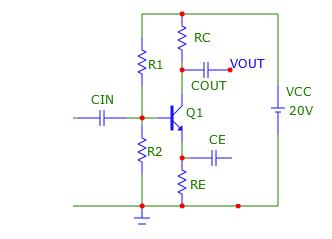
\includegraphics[scale=0.8]{circuito_setup.png}
	\caption{Montaggio iniziale del circuito}
	\label{f:setup}
\end{figure}

\begin{table}[h]
	\centering
	\begin{tabular}{*{3}{S[table-figures-decimal = 2, table-figures-uncertainty = 2]} *{4}{S[table-figures-decimal = 0, table-figures-uncertainty = 2]}} 
		{$R_1 [\si{\kohm}]$} & {$R_2 [\si{\kohm}]$} & {$R_C [\si{\kohm}]$} & {$R_E [\si{\ohm}]$} & {$C_{in} [\si{\nano\farad}]$} & {$C_{out} [\si{\nano\farad}]$} & {$C_E [\si{\micro\farad}]$} \\
		\hline 
		178.0 (15)	&	17.54 (15)	&	9.98 (9)	&	989 (9)	&	238 (12)	&	103 (4)	&	100 (10)	\\ 
	\end{tabular} 
	\caption{Valori misurati per i componenti del circuito}
	\label{t:misure_setup}
\end{table}

Dopo aver misurato i componenti (misure riassunte in \tab{misure_setup}), è stato montato il circuito come in \fig{setup}, usando il generatore per fornire $V_{cc}  =\SI{20 \pm .2}{\V}$.
Con l'ipotesi che questo circuito mantenga il transistor in regime attivo (che dal grafico delle curve caratteristiche fornito nella scorsa esperienza sembrerebbe ragionevole,
anche se la retta di carico non interseca nessuna curva relativa a correnti di base che ci attendiamo),
e dunque valgano $I_c = h_{FE} I_b$, $V_{BE} \approx \SI{0.60(5)}{\V}$, si sono stimate tensioni e correnti di funzionamento del circuito.
Questi valori attesi sono confrontati coi valori misurati (direttamente nel caso delle tensioni $V_c, V_e, V_b$, mentre le altre grandezze sono ricavate dalle misure di quest'ultime) in \tab{attesi-misure}.
L'accordo è generalmente buono, e in particolare è verificata l'ipotesi di regime attivo, il che ci permette di usare il circuito come amplificatore, come ci siamo preposti.

\begin{table}[h]
	\centering
	\begin{tabular}{ >{$}l<{$} | *{2}{S[table-number-alignment = center-decimal-marker]}}
			& {\hspace{30pt} Stimato} & {\hspace{30pt} Misurato} \\
		\hline
		I_b \ [\si{\uA}]	& 	6.2 (3)	&	7.1 (21)	\\
		V_c \ [\si{\V}]		&	9.0 (5)	&	9.12 (8)	\\
		V_e \ [\si{\V}]		&	1.10 (5)	&	1.100 (8)	\\
		V_b \ [\si{\V}]		&	1.69 (1)	&	1.68 (2)	\\
		V_{BE} \ [\si{\V}]	&	0.60 (5)	&	0.58 (2)	\\
		V_{CE}^Q \ [\si{\V}]	&	7.9 (5)	&	8.02 (8)	\\
		I_c^Q \ [\si{\mA}]	&	1.10(5)	&	1.09 (2)	\\
	\end{tabular}
	\caption{Confronto dei valori attesi con quelli misurati}
	\label{t:attesi-misure}
\end{table}

Concentrandoci sul partitore formato da $R_1$ e $R_2$, si ha per le rispettive correnti: $I_1 = \SI{104.9(14)}{\uA}$, $I_2 = \SI{95.8(14)}{\uA}$.
Poiché $I_2$ è nettamente maggiore di $I_b$ (e anche della corrente di base di saturazione, che dal grafico delle curve caratteristiche risulta minore \SI{20}{\uA}, forse vicina a \SI{10}{\uA}),
possiamo concludere che il partitore avrà un comportamento rigido nel corso dell'esperienza,
probabilmente mantenendo la sua "stiffness" anche quando ci si avvicina al regime di saturazione.

